\section{Mobile networks and security}

\question{Which vulnerability in the GSM network does the Stingray leverage?}
\begin{checkboxes}
    \CorrectChoice It exploits the fact that only the MS must authenticate in GSM.
    \choice It mounts a brute-force attack to recover the Ki and then decrypt all communications.
    \choice It uses the weaknesses in the A3/A8/A5 algorithms to mount a MITM attack.
    \choice It uses jamming to force a MS to connect to a rogue BS.
    \choice None of the other options.
\end{checkboxes}

\question{Which of the following are 2G vulnerabilities?}

\question{What are the main security issues in SS7 (Signaling System No. 7)?}
\begin{checkboxes}
    \CorrectChoice Caller ID spoofing and call redirection.
    \CorrectChoice Interception of SMS messages and phone calls.
    \CorrectChoice Location tracking of mobile devices.
    \choice Unauthorized access to subscriber billing information.
    \choice None of the other options.
\end{checkboxes}

\question{The SS7 signalling network is a protocol that}
\begin{checkboxes}
    % Source: google doc, verified
    \CorrectChoice Uses a datagram network to exchange signaling messages
    \CorrectChoice Uses out-of-band signalling approach so that messages are sent on a separate network than the telephone network.
    \choice Is a circuit-switched technology to setup, manage, and tear-down communications in the telephone network.
    \choice Is based on the ISO-OSI reference layer.
    \choice None of the other options.
\end{checkboxes}

\question{What is the purpose of paging and location areas in mobile networks?}
\begin{checkboxes}
    \choice To seamlessly transfer an active call or data session from one cell to another.
    \CorrectChoice To efficiently locate and notify a mobile device of an incoming call or message by dividing the network into smaller areas.
    \CorrectChoice Paging allows the BSC to locate the cell the MS is currently connected to.
    \choice To limit the MS power consumption so that it can sleep while not involved in any communications.
    \choice None of the other options.
\end{checkboxes}

\question{What is the difference between the Visitor Location Register (VLR) and the Home Location Register (HLR) in GSM networks?}
\begin{checkboxes}
    \CorrectChoice The VLR is a temporary database that stores information about subscribers currently roaming in the coverage area, while the HLR is a permanent database that contains detailed subscriber information and is maintained by the subscriber's home network.
    \choice The VLR handles billing and account information for roaming subscribers, while the HLR manages encryption keys and authentication data.
    \choice The VLR is responsible for managing voice call routing, while the HLR handles data transmission services.
    \choice The VLR stores the IMSI and Ki keys, while the HLR stores the subscriber's phonebook and SMS messages.
    \choice None of the other options.
\end{checkboxes}


\question{
    Consider the GSM Authentication Protocol timeline shown below:
\begin{figure}[H]
    \center
    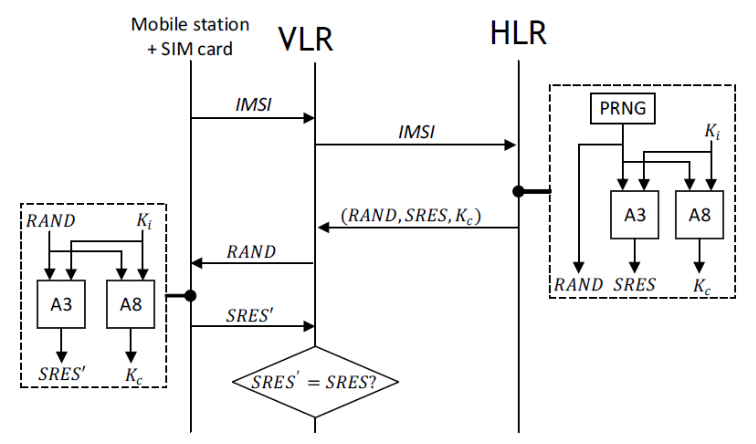
\includegraphics[width=0.7\textwidth]{images/GSM_auth.png}
\end{figure}
Associate the correct information to the correct number:
}
\begin{solution}
    \begin{enumerate}
        \item The MS sends the IMSI to the Visitor Location Register
        \item The Visitor Location Register forwards the subscriber IMSI to the Home Location Register
        \item Generates (RAND, SRES, Kc) and send them to the VLR
        \item Forwards RAND to MS
        \item Computes SRES' and send it to the VLR
        \item Compares SRES and SRES'
        \item Ki
        \item Kc
    \end{enumerate}
\end{solution}

\question{What is the primary purpose of handover in mobile networks?}
\begin{checkboxes}
    \choice To encrypt voice and data transmissions for secure communication.
    \choice To seamslessy transfer an active call or data session from one mobile teriminal to another.
    \choice To manage billing and account information for mobile subscribers when they move between to Base Stations.
    \choice To increase the data transmission speed betwen mobile devices.
    \CorrectChoice None of the other options.
\end{checkboxes}

\question{What are the main components involved in the GSM authentication process?}
\begin{checkboxes}
    \CorrectChoice SIM card, Authentication Center (AuC), and Home Location Register (HLR).
    \choice Mobile Equipment (ME), Visitor Location Register (VLR), and Base Transceiver Station (BTS).
    \choice Mobile Station (MS), Base Station Subsystem (BSS), and Network Switching Subsystem (NSS).
    \choice Mobile Management Entity (MME), Serving Gateway (SGW), and Packet Data Network Gateway (PGW).
    \choice None of the other options.
\end{checkboxes}

\question{Associate the correct definition to the correct component in the GMS architecture}
\begin{solution}
    % Source: google doc
    \begin{itemize}
        \item \textbf{Mobile Switching Centre:} Includes all control and signalling functions for managing calls and mobility
        \item \textbf{User Equipment:} The user's mobile device. It includes a Terminal Equipment (TE) and a Subscriber Identity Module (SIM) card
        \item \textbf{Base Station Controller:} Implements higher layers protocols and manages all transmission resources of the connected BTSs
        \item \textbf{Base Transceiver Station:} Manages physical layer connections with the UEs and the BSC
        \item \textbf{Gateway MSC:} Connects the mobile network to the external telephone networks. It implements all signalling interworking functions 
    \end{itemize}
\end{solution}

\question{What are the advantages and disadvantages of having small or larger cells in mobile networks?}
\begin{checkboxes}
    \choice Small cells are more expensive to deploy and maintain compared to larger cells, which are cheaper and more energy-efficient.
    \choice None of the other options.
    \choice Small cells are only suitable for urban areas, while larger cells can only be used in rural areas.
    \choice Small cells reduce interference and improve signal quality, whereas larger cells are prone to higher levels of interference and degraded signal quality.
    \CorrectChoice Small cells provide higher capacity and better coverage in dense areas but may require more frequent handovers as users move, while larger cells cover wider areas with fewer handovers but might have lower capacity in dense environments.
\end{checkboxes}

\question{Which of the following technologies are used in 4G networks to enhance security?}
\begin{checkboxes}
    \CorrectChoice Advanced Encryption Standard (AES) for data encryption.
    \CorrectChoice Non-Access Stratum (NAS) security for signaling protection.
    \choice Implementation of advanced firewall technologies at the network core.
    \choice Temporary Mobile Subscriber Identity (TMSI) for user anonymity.
    \choice None of the other options.
\end{checkboxes}

\question{What is the difference between the IMSI and the TMSI in mobile networks?}
\begin{checkboxes}
    \choice The IMSI identifies the mobile device, while the TMSI identifies the subscriber's location area.
    \choice The IMSI is a randomly generated number used for secure authentication, while the TMSI is a fixed identifier stored on the SIM card.
    \CorrectChoice The IMSI is a unique identifier assigned to a mobile subscriber by the home network, while the TMSI is a temporary identifier used to protect the subscriber's identity during communications with the network.
    \choice The IMSI is used for billing and account management, while the TMSI is used for data encryption.
    \choice None of the other options.
\end{checkboxes}

\question{How does the GSM network authenticate a subscriber using the SIM card?}
\begin{checkboxes}
    \choice By requiring the subscriber to enter a personal identification number (PIN).
    \choice By sending a challenge (RAND) to the Authentication Center, which generates a response (SRES) using the Ki key.
    \choice By sending a challenge (RAND) to the SIM card, which generates a response (SRES) using the TMSI key.
    \choice By sending a challenge (RAND) to the SIM card, which generates a response (SRES) using the IMSI key.
    \CorrectChoice None of the other options.
\end{checkboxes}

\question{Associate the correct answer to each of the following terms:}
\begin{solution}
    \begin{itemize}
        \item UMTS Multiple Access is based on \fillin[Code Division Multiple Access][2in]
        \item UMTS network supports \fillin[both circuit- and packet- switching technologies][2in]
        \item 4G networks supports \fillin[only packet-switching technologies][2in]
        \item Original GMS networks supports \fillin[only circuit-switching technolgies][2in]
        \item GMS Multiple Access is based on \fillin[Time Division and Frequency division Multiple Access][2in]
    \end{itemize}
\end{solution}

\question{What is the purpose of the Ki key stored on a SIM card?}
\begin{checkboxes}
    \choice To identify the SIM card and its subscriber's information.
    \choice To store the subscriber's phonebook and SMS messages in encrypted format.
    \choice To encrypt voice and data transmissions over the mobile network.
    \CorrectChoice To authenticate the SIM card to the mobile network.
    \choice None of the other options.
\end{checkboxes}

\question{Associate the correct definition to the following UMTS security features:}
\begin{solution}
    % source: google doc
    \begin{itemize}
        \item \textbf{Network domain security}: The set of security features that enable nodes in the provider domain to exchange signalling data securely.
        \item \textbf{Visibility and configurability of security}: The set of features to inform the user whether a security feature is in operation or not.
        \item \textbf{User domain security}: The set of security features that secure access to mobile stations.
        \item \textbf{Network access security}: The set of security features that provide users with secure access to 3G services.
        \item \textbf{Application domain security}: The set of security features that enable applications in the user and the provider domain to exchange messages securely.
    \end{itemize}
\end{solution}


\question{Considering the GSM A5 algorithm used to provide confidentiality in GMS, which of the following claims are correct?}
\begin{checkboxes}
    % Source: google doc
    \CorrectChoice It uses multiple Linear Feedback Shift Registers which are clocked to increase the entropy of the keystream.
    \CorrectChoice It uses 54 bits long likely to allow national agencies to decrypt communications.
    \CorrectChoice There were two versions of the A5 algorithm: one for usage in western countries, one for export outside western countries.
    \CorrectChoice It uses the Cypher Key Kc and the Frame Number FN to compute the encryption key stream.
    \choice None of the other options.
\end{checkboxes}

\question{What is the difference between user signaling and network signaling in mobile networks?}
\begin{checkboxes}
    \choice User signaling is responsible for establishing and maintaining connections, while network signaling manages the subscriber's phonebook and SMS messages.
    \choice User signaling includes all types of data transmission between users, while network signaling is used solely for billing and accounting purposes.
    \choice User signaling is used to manage handovers between cells, while network signaling is used to encrypt data transmissions.
    \CorrectChoice User signaling allows the setup for the transmission of user data such as voice and text messages, while network signaling involves the exchange of control information to manage the network and ensure proper communication.
    \choice None of the other options.
\end{checkboxes}

\question{What is the concept of cellular coverage in mobile networks?}
\begin{checkboxes}
    \choice The range within which a mobile device can connect to a single cell tower and receive a signal.
    \choice The maximum data transmission speed that can be achieved within a specific area of the network.
    \CorrectChoice The area served by a cellular network where users can make and receive calls, use data services, and move without losing connection.
    \choice The method by which multiple cell towers coordinate to provide seamless connectivity to a mobile device.
    \choice None of the other options.
\end{checkboxes}